\chapter{Proposed System Architecture}\makeatletter\def\@currentlabel{3}\makeatother
\label{chap2}
\lhead{\textbf{CHAPTER 2.} \textit{Proposed System Architecture}}
 This chapter provides a comprehensive blueprint of the \textit{zkpoex} framework.  
We begin with a concise overview of the \texttt{research methodology} employed to survey relevant literature and distil the design requirements.  The discussion then introduces the \ref{risc0_zkVM} (zkVM) that underpins succinct proof generation, followed by an examination of the \ref{rustevm} (Rust EVM) and the interoperability layer that bridges these two environments.  The chapter concludes with a detailed walkthrough of the exploit-execution pipeline, illustrating how each component cooperates to produce a verifiable receipt. After reading all of this chapter, you can view a schematic of the workflow of the first release of \textit{zkpoex} (\texttt{v0.1.0}) in Figure \ref{fig:zkpoexSchem}.

\begin{figure}[h]
    \centering
    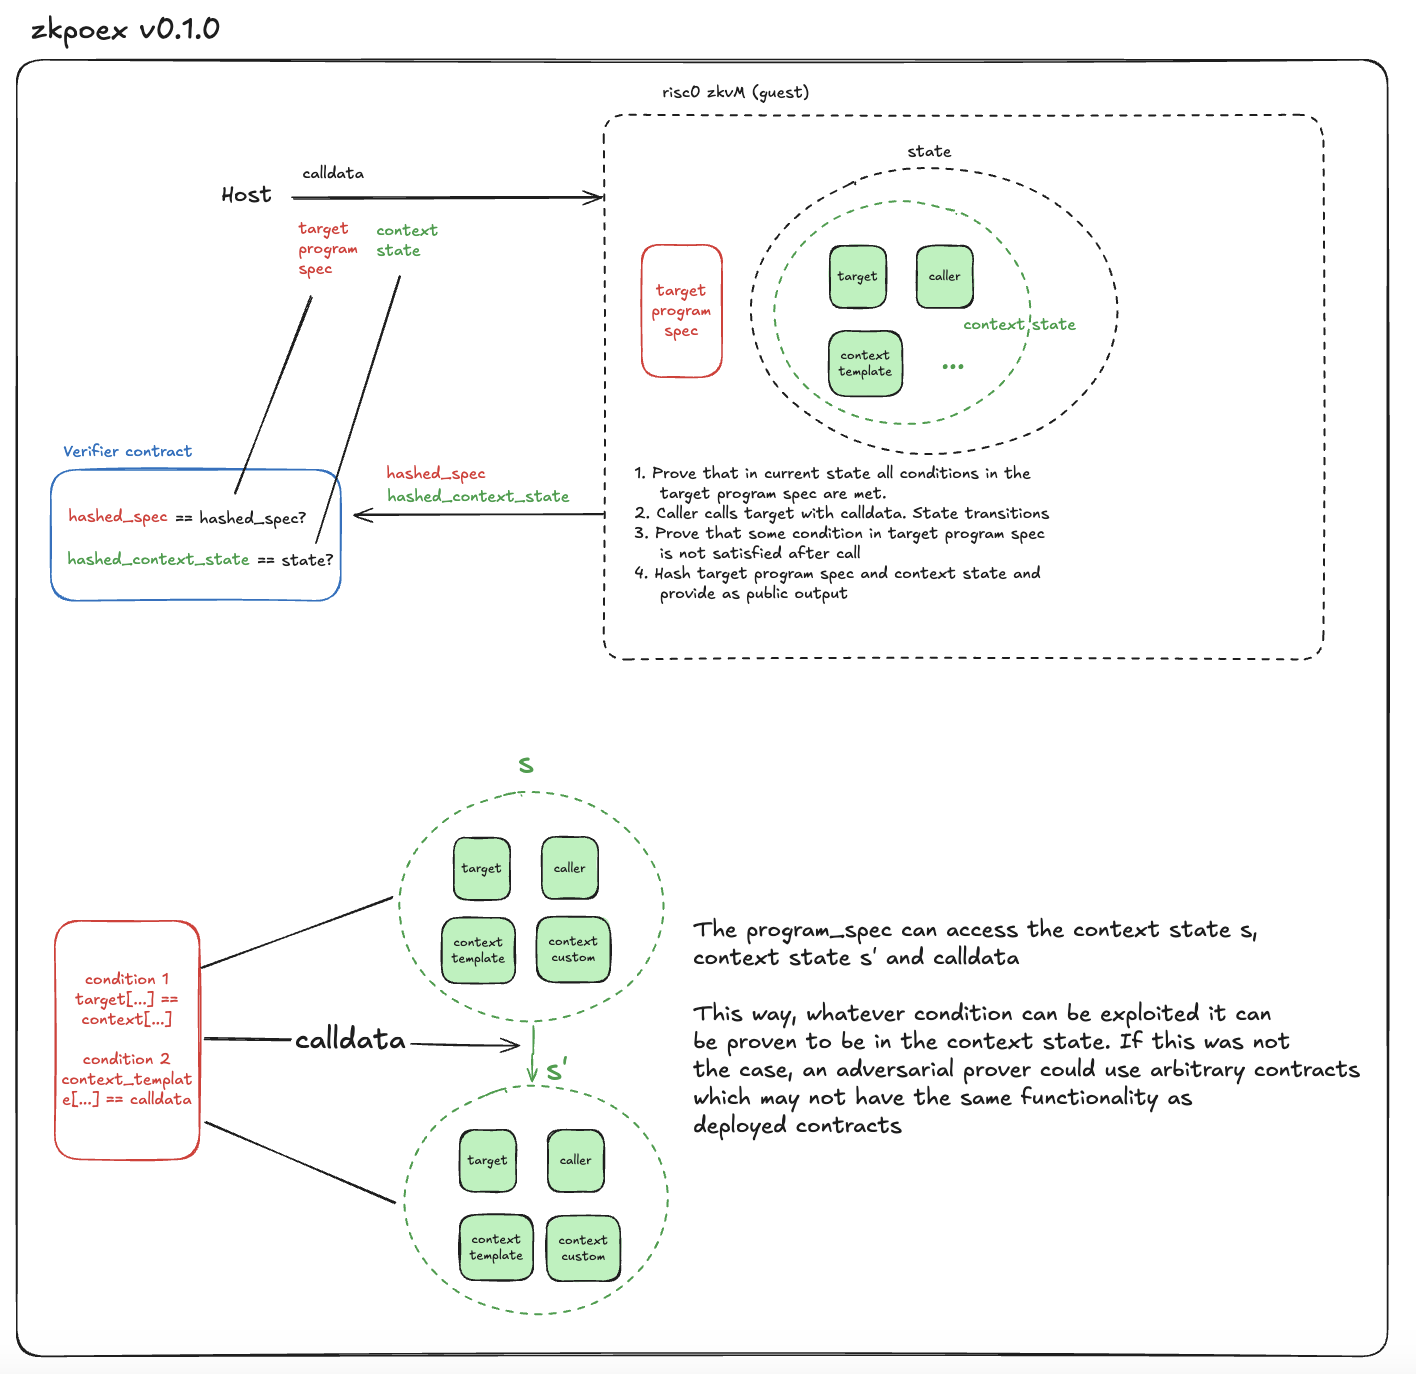
\includegraphics[width=1\linewidth]{Images/Chap2/zkpoex-v0.1.0.png}
    \caption{A schematic of the \textit{zkpoex} workflow \cite{zkpoex_docs}}
    \label{fig:zkpoexSchem}
\end{figure}

\section{Overview of the System}
The \textit{zkpoex} project couples a conventional host process with a guest program that runs inside a RISC Zero zero-knowledge virtual machine (zkVM). In addition, a Rust Ethereum Virtual Machine (Rust EVM) interpreter is launched in the guest program to simulate smart-contract attacks.
The host supplies public context: chain height, gas price, account state hashes, together with confidential artefacts such as the exploiter bytecode and crafted calldata.  
The guest, compiled to RISC-V, replays a single Ethereum transaction inside the Rust EVM and emits a receipt through the \textit{zkpoex} prover whose journal binds the initial public state, the post-execution state root, and a commitment to every hidden input.  

This separation lets an auditor (or private projects) convince a verifier that, given a \textit{calldata}, to prove an exploit, he must first define a set of conditions called \textit{program\_specifications}. \textit{zkpoex} uses this specification to verify whether a state transition invalidates any conditions in the smart contract. You can read a formal explanation of this in section \ref{sec:core-problem}

At a higher level of abstraction, the \textit{zkpoex} system can be viewed as two principal components: \ref{zkpoex_prover} and \ref{zkpoex_scOwner}. Before delving into these main components, we will explore some key concepts introduced in \texttt{zkpoex}:

\begin{itemize}
    \item \ref{zkpoex_contstate},
    \item \ref{zkpoex_progspec}.
\end{itemize}

\subsection{Context State}\makeatletter\def\@currentlabel{Context State}\makeatother\label{zkpoex_contstate}

The \texttt{context\_state} is a compact snapshot of the on-chain world that the prover is allowed to touch.  
Each entry in the top-level array represents one Ethereum account and is encoded as a plain JSON object:

\begin{itemize}
    \item \textbf{address}: 20 byte address, left-padded to 40 hex characters; serves as the Merkle-Patricia key.
    \item \textbf{nonce}: transaction counter, stored as a decimal string to avoid surprises when serialising.
    \item \textbf{balance}: Wei balance, again string-encoded so that very large values survive round-trips.
    \item \textbf{storage}: sparse map \verb|slot → value| where both keys and values are 32-byte hex words; only touched slots are listed, which keeps the witness small.
    \item \textbf{code}: run-time bytecode of the contract, hex-prefixed; an empty string marks an EOA.
\end{itemize}

During proof generation, the guest computes the Keccak256 Merkle root of this structure and exposes it in the journal.  
Because the contract owner supplies the state and becomes public, the prover cannot smuggle in a \texttt{favourable} pre-state; at the same time, limiting the snapshot only to the accounts of interest keeps the circuit lean and the proof time acceptable. 

\vspace{0.8em}

\subsection{Program Specifications}\makeatletter\def\@currentlabel{Program Specifications}\makeatother\label{zkpoex_progspec}

While \texttt{context\_state} is a simple, enumerable snapshot of the world, a
\texttt{program\_specification} is closer to a \texttt{behavioural contract}.  
It captures, in machine-readable form, the invariants that \texttt{must} continue to
hold for a contract, no matter which calldata the prover chooses.  
Because it encodes logical properties rather than raw data, the file is
necessarily more articulated; the subsection is therefore slightly longer.

A specification is an \texttt{array of method descriptors}.  
Each descriptor binds one function selector to a set of post-execution
predicates and an (optional) ABI schema:

\begin{itemize}
  \item \textbf{method\_id:} Four-byte selector \(\text{keccak}(\text{signature})[0..4]\).
        Only EVM calls whose calldata starts with this prefix are analysed by the
        zkVM.
  \item \textbf{conditions:} An ordered list of predicates that must evaluate to
        \textsc{true} \texttt{after} the call returns.  
        Predicates are written in a DSL whose atomic form is
            \begin{quote}
    \verb|{ "Fixed": { "k_s": "<path>", "op": "<Op>", "v": "<value>" } }|
            \end{quote}
        where:

        \begin{itemize}
           \item \verb|k_s| selects either
                 \texttt{<addr>.balance} or
                 \texttt{<addr>.storage.<slot>};
           \item \verb|op| is one of
                 \texttt{Eq}, \texttt{Ne}, \texttt{Gt}, \texttt{Ge},
                 \texttt{Lt}, \texttt{Le};
           \item \verb|v| is a constant against which the post-state is compared.
        \end{itemize}
        The zkVM walks the list; the \texttt{first} violated predicate is enough to declare an exploit and halt the trace.
  \item \textbf{arguments:} ABI-typed parameter list.  
        It exists solely so that front-end tooling and fuzzers can craft valid
        calldata; the verifier contract does not inspect this field.
\end{itemize}

In practice, the contract owner publishes the current bytecode, its
\texttt{context\_state}, and the \texttt{program\_specification} on-chain,
locks a bounty, for instance, and waits.  
A white-hat feeds the same artefacts to \textit{zkpoex}, searches for calldata
that breaks at least one predicate, and produces a zero-knowledge proof whose
journal commits to the \texttt{hash} of the specification, never to the exploit
input itself.  
If the verifier contract confirms that the committed hash matches the
canonical specification, funds are released, but the calldata remains private.


\subsubsection{Formal taxonomy of conditions}\label{zkpoex_formal_conditions}

From \cite{zkpoex_docs}: Let \(A = 2^{160}\) be the address space and \(V = 2^{256}\) the word space.
A \texttt{state} is a map \(s: A \rightarrow V\).

\paragraph{Fixed condition.}
\[
F_{s}(a,\,op,\,v)\;:=\;
\bigl(s(a)\;\text{\(op\)}\;v\bigr),\quad
a\in A,\;v\in V .
\]

\paragraph{Relative condition.}
Given a pre-state \(s\) and a post-state \(s'\):
\[
R_{s,s'}(a,\,op,\,a')\;:=\;
\bigl(s(a)\;\text{\(op\)}\;s'(a')\bigr),
\quad a,a'\in A .
\]

\paragraph{Specification.}
Let \(m(i, s)\) be the state transition induced by a method \(m\) on input
\(i\).  
A specification is a finite set
\[
S=\{(m, C_m)\},
\]
where \(C_m\) is a list of conditions attached to \(m\).
\(S\) is \texttt{valid} iff for every \(m,i\) and for every pre-state \(s\) the
post-state \(s'=m(i,s)\) satisfies all the associated conditions:
\[
\forall (m, C_m)\in S,\;\forall i,\;
\forall c\in C_m,\; c(s,s') = \textsc{true}.
\]

An exploit is a witness \(i_E\) such that some \(m\) turns a valid state into a
state where at least one \(c\in C_m\) is \textsc{false}.  
Producing a \textit{zk-STARK-to-SNARK} (you can see section \ref{proof_system} to deep in the RISC Zero's full proving stack) proof that attests this fact, without revealing \(i_E\), fulfils the bounty and enables rapid, privacy-preserving incident response.


\subsection{The \textit{zkpoex} Prover}\makeatletter\def\@currentlabel{The \textit{zkpoex} Prover}\makeatother
\label{zkpoex_prover}

Conceptually, the \textit{zkpoex} prover reuses the standard RISC Zero prover discussed in \ref{risc0_zkVM}, but tailors the workflow to an Ethereum-specific payload. At a high level, the prover finds an exploit in the owner's smart contract and generates a zero-knowledge proof of the exploit execution. To do so, it shows that it knows some calldata that can be used to call the contract such that it breaks the contract's \textit{program\_specification}. The prover can verify said proof and claim rewards automatically without the need for a third party. On-chain operations and all the technicalities will be discussed in more detail in \ref{chap3} Chapter.

\subsection{The Smart-Contract Owner}\makeatletter\def\@currentlabel{The Smart-Contract Owner}\makeatother
\label{zkpoex_scOwner}

The \textit{Smart-Contract Owner} in the \textit{zkpoex} vision is the actor that is responsible for:

\begin{itemize}
    \item Deploying the \textit{VerifierContract};
    \item Setting up the \textit{program\_specification};
    \item Defining the rewards in the \textit{VerifierContract} for the prover.
\end{itemize}

As mentioned in the first chapter of this thesis (\ref{contextMotivation}), the \textit{zkpoex} project wants to verify, in a totally trustless environment, that a smart-contract exploit exists without any leak of exploit details. To do so, the \textit{Smart-Contract Owner} needs to deploy the \textit{VerifierContract} of \textit{zkpoex}, which interacts, depending on the Ethereum network you are using, with the deployed Verifier of RISC Zero \cite{risc0_verifier}.

In our setting, the guest steps through an EVM interpreter, executes the target smart contract, and checks the run against a predetermined specification. Once the computation finishes and the zero-knowledge proof is produced, two public hashes are published: 
\begin{itemize}
    \item $\mathrm{Keccak256}(S)$, where $S$ is the \textit{program\_specification} in force;
    \item $\mathrm{Keccak256}(C)$, where $C$ is the hash of \textit{context\_state} data (such as other deployed contracts).
\end{itemize}

A sound proof alone is not sufficient. To ensure the guest really inspected the contract that is live on chain and did so under the current rules, the verifier recomputes each hash from today’s artefacts and compares. If the freshly derived hash of the specification differs from the advertised $\mathrm{Keccak256}(S)$, or the hash of \textit{context\_state} from $\mathrm{Keccak256}(C)$, the receipt is rejected. Such a discrepancy would signal that the proof targets outdated code or an obsolete specification. Only when every comparison coincides does the verifier accept the claim, confirming that the evidence truly pertains to the contract and specification currently deployed. After that, the \textit{VerifierContract} sends automatically the reward to the prover.



\section{The RISC Zero zkVM} \makeatletter\def\@currentlabel{RISC Zero zero-knowledge virtual machine}\makeatother
\label{risc0_zkVM}
The \texttt{RISC Zero} zero-knowledge virtual machine (you can find an explanation of what a zkVM is, in general, in section \ref{zkvm}) functions on a fundamental principle: a \textit{guest program}, utilizing a designated instruction set, is performed within a virtual machine environment, producing the appropriate proof.

As said in RISC Zero Docs: “The RISC Zero zkVM lets you prove correct execution of arbitrary Rust code. By allowing users to build zero-knowledge applications that leverage existing Rust packages, the RISC Zero zkVM makes it quick and easy to build powerful verifiable software applications.”\cite{risc0_zkvm}

In Figure \ref{fig:pipeline_RISC Zero}, you can see the components of a RISC Zero zkVM:

\begin{enumerate}
  \item \textbf{\ref{guestcode}}: the Rust routine whose execution will later be attested;
  \item \textbf{\ref{executor}}: runs the compiled binary and records the full execution trace;
  \item \textbf{\ref{prover}}: checks that trace step-by-step and compresses it into a proof;
  \item \textbf{\ref{receipt}}: the compact artefact that bundles the public journal and its zero-knowledge seal;
  \item \textbf{\ref{hostcode}}: the machine that is running the zkVM.
  
\end{enumerate}

\begin{figure}[h]
    \centering
    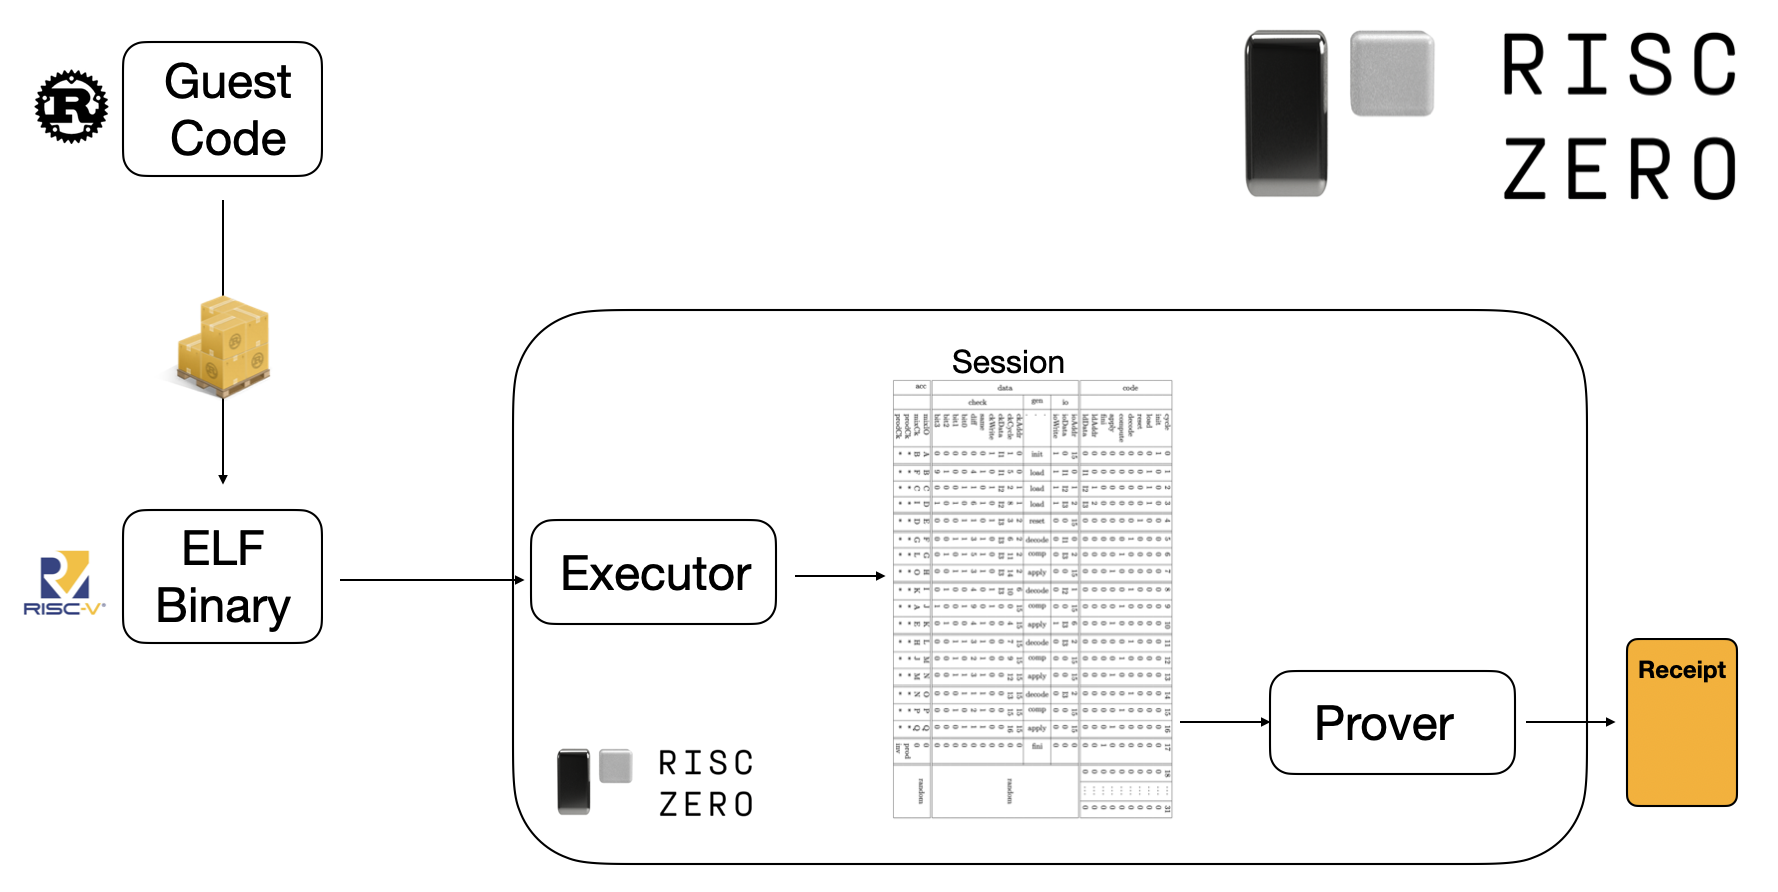
\includegraphics[width=1\linewidth]{Images/Chap2/risc0_flow.png}
    \caption{End-to-end proving pipeline in RISC Zero \cite{risc0_zkvm}}
    \label{fig:pipeline_RISC Zero}
\end{figure}

\subsection{The Receipt} \makeatletter\def\@currentlabel{Receipt}\makeatother
\label{receipt}
As noted in \cite{risc0_receipt}, a \textit{Receipt} (shown as a gold document in Figure \ref{fig:pipeline_RISC Zero}) is the artefact that the zkVM returns once your guest program finishes: it combines the programme’s public outputs, collected in the \textit{journal}, with a zero-knowledge proof called the \textit{seal}.  
Because the seal is a succinct validity proof, anyone can verify without re-executing the code that the journal was produced by the expected image ID and that every step of execution was sound.

A typical workflow is therefore straightforward.  
\begin{enumerate}
  \item Alice runs the guest, producing a receipt.  
  \item She forwards that receipt to Bob.  
  \item Bob first reads the public results through \texttt{receipt.journal};  
  \item Bob then calls \texttt{receipt.verify()}, gaining cryptographic assurance that:
        \begin{itemize}
          \item the computation was carried out faithfully;  
          \item the guest binary matched the agreed image ID.  
        \end{itemize}
\end{enumerate}

Receipts are ordinary Rust structures, but they can be serialised with any \texttt{serde}\footnote{A generic serialization/deserialization framework for Rust} compatible format.


\subsection{The Guest Code}\makeatletter\def\@currentlabel{Guest Code}\makeatother
\label{guestcode}

The \textit{Guest Code} (shown with the Rust logo in Figure \ref{fig:pipeline_RISC Zero}) is the self-contained Rust routine that the zkVM will actually execute and prove.  
Once compiled to a RISC-V \textit{ELF binary} (indicated by the RISC-V logo in Figure \ref{fig:pipeline_RISC Zero}), its initial memory image is hashed to a unique \texttt{Image ID}.  
That identifier later lets any verifier check that a receipt truly originated from the expected binary; no source code is strictly required, only the ELF (or its Image ID) needs to be shared.  

But why does this determinism matter? Because every byte of the ELF contributes (via the memory image) to the Image ID, even seemingly innocuous differences like timestamps, debug sections, or compiler versions would change the hash and break verification.

\subsection{The Executor}\makeatletter\def\@currentlabel{Executor}\makeatother
\label{executor}

The \textit{Executor} is the portion of the zkVM responsible for generating the \textit{execution trace}. The \textit{Executor}, basically, runs the program inside the RISC Zero environment and records a full execution \textit{Session} (or execution trace), displayed as a tabular trace of instructions, registers, and memory activity. From \cite{risc0_key_terminology}: “Each row describes a complete snapshot of the state of the zkVM at a given moment in time. The width of the execution trace relates to the number of registers/components in the machine, and the length of the execution trace relates to the number of clock cycles\footnote{ From \cite{risc0_key_terminology}: “The smallest unit of compute in the zkVM circuit, analogous to a clock cycle on a physical CPU. The complexity of a guest program's execution is measured in clock cycles as they directly affect the memory, proof size, and time performance of the zkVM”.} of the program's execution”. The \textit{Prover} will check the validity of that recorded \textit{Session} after.

\subsection{The Prover}\makeatletter\def\@currentlabel{Prover}\makeatother
\label{prover}

The \textit{Prover} is the portion of the zkVM that executes and proves a \textit{guest} program, thereby constructing a \textit{receipt}. As shown in Figure \ref{fig:pipeline_RISC Zero}, the \textit{Prover} takes the recorded \textit{Session} and checks its validity. A valid trace means that the \textit{ELF binary} was faithfully executed according to the rules of the RISC-V instruction set architecture. In RISC Zero, there are two types of \textit{Provers}:

\begin{itemize}
    \item \textbf{Local Prover:} Generates proofs locally.
    \item \textbf{Remote Prover:} Uses a remote service called \textit{Bonsai}\cite{risc0_remote_proving}.
\end{itemize}

\subsection{The Host Code}\makeatletter\def\@currentlabel{Host Code}\makeatother
\label{hostcode}

From \cite{risc0_host}, the host is an untrusted agent that sets up the zkVM environment and handles inputs/outputs during execution. Although not seen in Figure \ref{fig:pipeline_RISC Zero}, it is still an important component of a RISC Zero zkVM application. Before any proving begins, the host first prepares a dedicated execution environment for the \textit{Executor}.  This sandbox collects every run-time parameter configuration flag, input buffers, and any other settings, and forms the sole communication channel between host and guest. Once the environment is ready, the host launches the \textit{Prover}. The resulting receipt, containing both the public journal and its zero-knowledge seal, as said before, can then be forwarded to a third party, who may verify it independently without rerunning the computation or trusting the original host.

\section{Proof System Used}\label{proof_system}

The zero-knowledge layer adopted by \textit{zkpoex} is precisely the
\texttt{RISC Zero proof stack} \cite{risc0_proving_stack}.
It compresses the full execution trace discussed in
\ref{risc0_zkVM} into a single on-chain verifiable artefact, balancing three
conflicting goals: transparent setup, fast GPU proving, and tiny verifier
costs. The illustrative figure for this chapter and its subsections is Figure \ref{fig:proving_stack}. 

\begin{figure}[h]
    \centering
    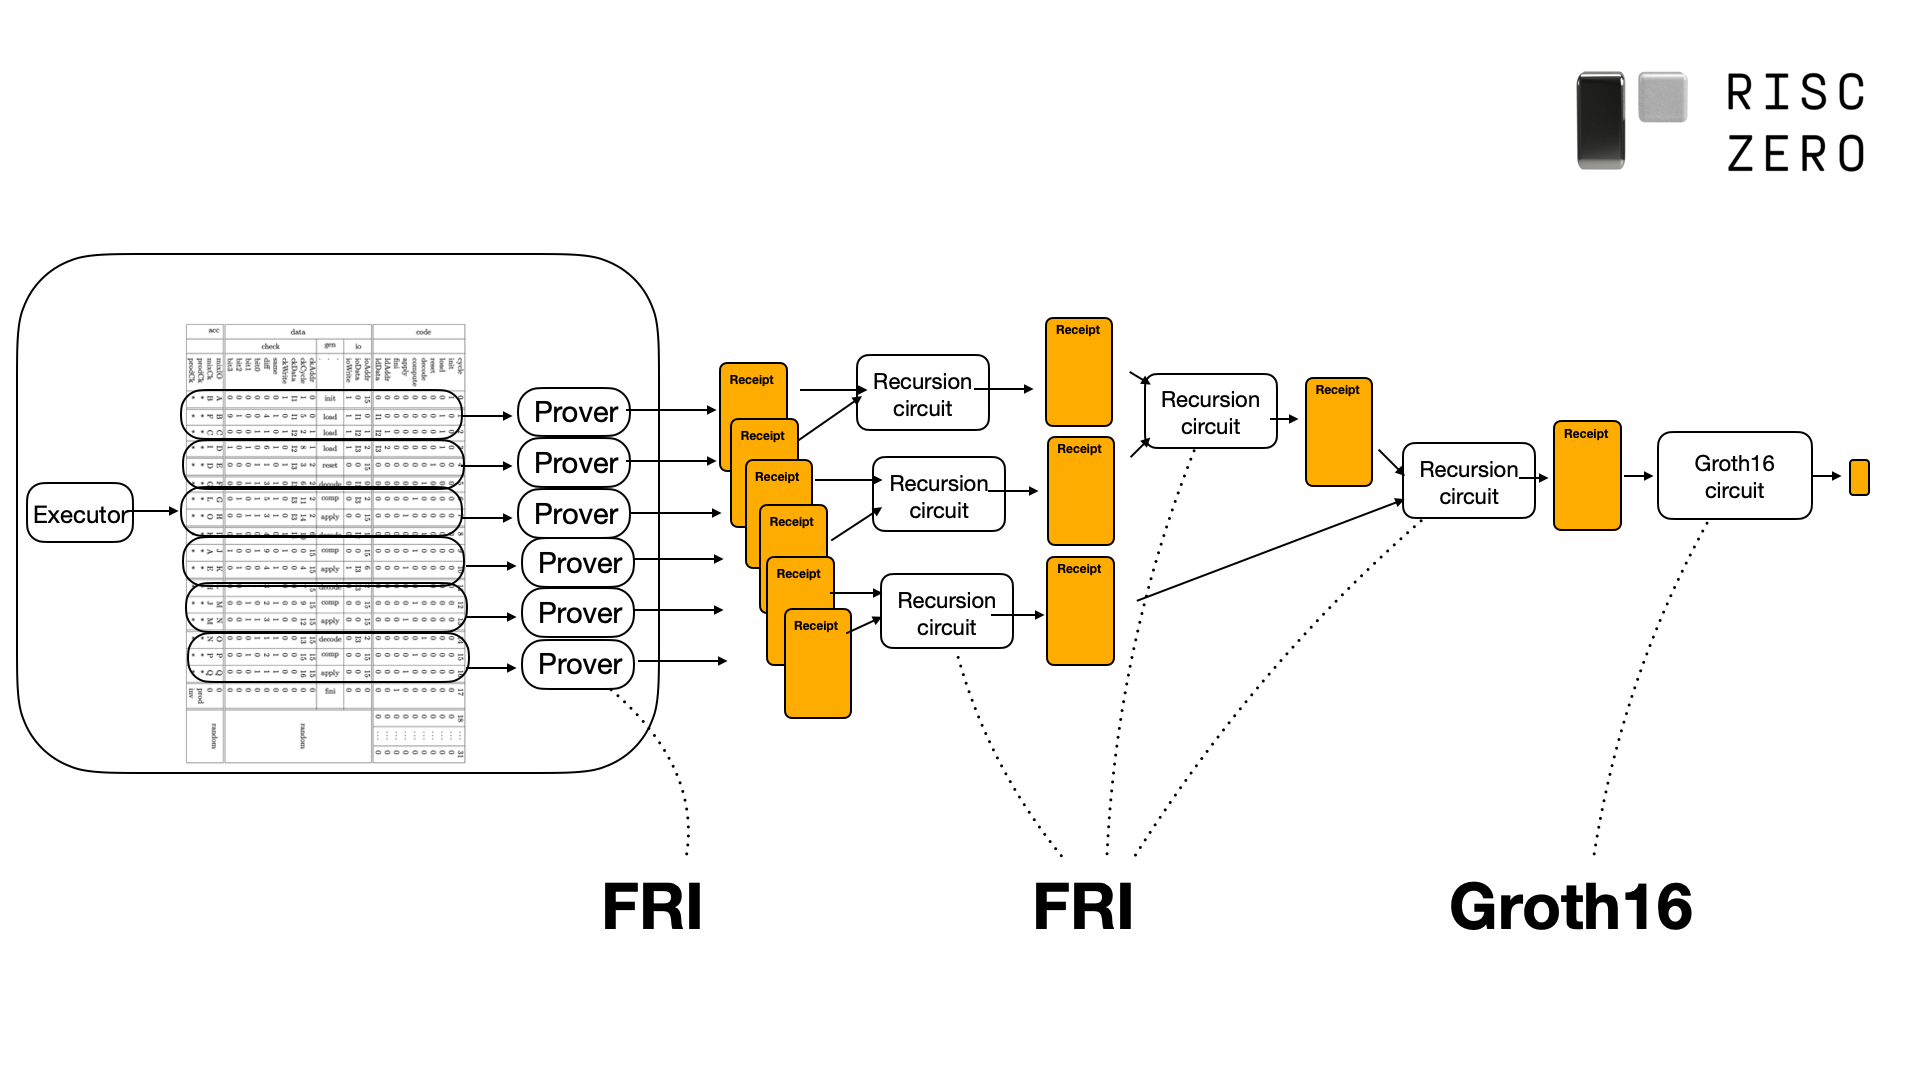
\includegraphics[width=1\linewidth]{Images/Chap2/proofStackRisc0.png}
    \caption{The RISC Zero's full proving stack \cite{risc0_proving_stack}}
    \label{fig:proving_stack}
\end{figure}

\subsection{Four layer architecture} \label{risc0_4layer}
Before diving into the individual stages, it is helpful to view the RISC Zero
proof stack as a \texttt{pipeline}: From \cite{0stark_blog}: raw execution traces enter at the top, while a
concise, on-chain–friendly SNARK emerges at the bottom.  The transformation is
carried out in four logical layers, each building on the previous one and
serving a distinct purpose in the compression hierarchy.

\begin{enumerate}
  \item \textbf{Execution:}  
        The guest routine is run natively, but thanks to
        continuations, the VM may pause whenever memory, time, or proof
        limits are met, yielding a sequence of \texttt{segments}.
  \item \textbf{Segment proving:}  
        With \texttt{0STARK}, each section is independently verified; it is a 
        STARK dialect, whose arithmetisation is AIR-based and whose commitment scheme relies on the FRI low-degree protocol over the 31-bit
        \texttt{Baby Bear} field. 0STARK was engineered for
        massive horizontal scalability on GPU clusters and currently delivers
        about 98 bits of concrete security.
  \item \textbf{Aggregation proving:}  
        The many segment receipts are fed into a dedicated \texttt{recursion
        circuit}, itself expressed in 0STARK, which folds them into a single
        STARK proof. Because verification is executed inside the same proof
        system that created the segments, recursion remains GPU-friendly, and
        keeps prover costs sub-quadratic in the total trace length.
  \item \textbf{STARK-to-SNARK compression:}  
        Finally, the aggregated STARK is verified inside a small
        \texttt{Groth16} circuit. The result is a  succinct elliptic-curve
        SNARK, only a few hundred bytes, whose verification gas on Ethereum fits
        comfortably below typical block limits, making it practical for the
        \texttt{VerifierContract} referenced in \ref{zkpoex_scOwner}.
\end{enumerate}

\subsection{Design rationale}
The layering outlined above is not arbitrary.  Each component has been chosen to reconcile transparency, prover throughput, and on-chain efficiency, three properties that rarely coexist in a single proof system.  The considerations below summarise why the RISC Zero team settled on this particular combination of STARKs, recursion, and Groth16.

\paragraph{Transparent trust model:}
All layers, except the final Groth16 step, are STARK-style and therefore do not require \texttt{trusted setup}; the only structured reference string left is the universal SRS\footnote{A structured reference string (SRS) is the public parameter set produced in a one-time trusted-setup ceremony; Groth16 needs a universal SRS, whereas STARKs require none.} provided with Groth16, which can be reused by any application. 

\paragraph{Proof size vs. prover cost:}
While a pure STARK would avoid elliptic curves altogether, its proof would weigh hundreds of kilobytes.  Compressing the proof through Groth16 trades a one-off trusted setup for two decisive advantages: 
\begin{enumerate}[label=(\roman*)]
    \item A ~1 kB receipt;
    \item A verifier that fits into a single precompile on most EVM chains.
\end{enumerate}

\paragraph{GPU parallelism:}
Running FRI over a small prime field allows the prover to exploit SIMD arithmetic, and FFT kernels are already optimised for graphics workloads. Recursion is structured so that each segment can start proving as soon as its trace is available, the executor never has to wait for the last segment to finish before dispatching earlier ones, maximising cluster utilisation.

\subsection{Implications for \textit{zkpoex}}

Embedding \textit{zkpoex} in this proof stack yields concrete benefits:

\begin{itemize}
  \item \textbf{Auditability:}  Anyone can verify the final Groth16 receipt on-chain and be certain that the underlying STARKs were produced from the exact \textit{context\_state} and \textit{program\_specification} hashes committed in the journal, see the hash-matching logic in \ref{zkpoex_scOwner}.
  
  \item \textbf{Privacy:}  The aggregation circuit reveals only the public journal; all intermediate segment traces, including the exploiter’s calldata, remain hidden from both the bounty sponsor and the chain.
  
  \item \textbf{Scalability:}  Thanks to continuations and GPU-centric 0STARK, even complex EVM transactions (or entire blocks) can be proven within the time and memory budget of commodity cloud instances.
  
\end{itemize}

In short, the RISC Zero proof system equips \textit{zkpoex} with a battle-tested,
transparent and economically viable foundation, ensuring that every exploit
proof produced by \ref{zkpoex_prover} can be verified
efficiently and trustlessly on any EVM-compatible network.

\section{The Rust EVM}\makeatletter\def\@currentlabel{Rust-based Ethereum Virtual Machine}\makeatother
\label{rustevm}

A zero-knowledge executor that must replay arbitrary Ethereum bytecode inside a Rust-centric zkVM, like the RISC Zero, one gains a decisive advantage from an interpreter developed in the same language.  The \textit{Rust EVM} crate\footnote{In Rust, a \emph{crate} is the smallest compilation unit, a library or binary package published on \texttt{crates.io} and imported with \texttt{cargo}.} maintained by the Rust-Ethereum working group offers a compact, no-\textit{unsafe} implementation that meets this requirement\cite{rust_evm_crate}.  The following pages explain why this choice was preferred over C++, Go, or JavaScript engines, describe the interpreter’s essential building blocks, and clarify the adjustments applied for \textit{zkpoex}.  For the reader’s convenience, the discussion refers back to the execution semantics introduced in \ref{ethOverview}.

\subsection{Why a Rust interpreter}

The first reason is tool-chain homogeneity.  Every layer of the RISC Zero stack, guest SDK, host interface, proof gadgets, already relies on Rust; by using a Rust interpreter,r the project avoids foreign-function interfaces, keeps the guest binary small, and reaps deterministic builds through a single \texttt{cargo} command.  Memory safety follows as a corollary: ownership rules guarantee that no dangling pointer or data race can corrupt the trace, an essential property because a crash inside the zkVM would render the proof invalid. Equally important is the interpreter’s modular approach to hard forks. Gas tables and pre-compile behaviour vary from Frontier to Shanghai, yet the crate encapsulates these differences behind “handler” traits so that \textit{zkpoex} can select the appropriate ruleset at compile time with no change to opcode semantics. Finally, the code base is deliberately lightweight; apart from primitive numeric types and hashing utilities, there are no heavy external dependencies, which simplifies static linking into the guest image and minimizes proof size.

\subsection{Interpreter design}

At run time, the engine revolves around three subsystems.  A tight dispatch loop maps opcodes to their semantic handlers while accounting for fork-specific gas schedules; whenever the remaining gas falls below a safety margin, the zkVM yields, allowing the host to seal the current segment before memory usage grows. State access is mediated by a host trait that abstracts balance, storage, and code look-ups.  In \textit{zkpoex}, this trait is backed by a Merkle-tree store pre-seeded from the \texttt{context\_state}; every leaf that the interpreter touches is logged in the journal so the verifier can recreate the same root.  Cold-versus-warm bookkeeping, introduced by \texttt{EIP-2929}, is maintained by an in-guest cache whose final digest appears in the receipt, ensuring that gas metering remains deterministic on-chain.

\subsection{Tailoring the engine to \textit{zkpoex}}

Deterministic gas accounting is the foremost requirement: all host-dependent look-ups are performed in-guest and their outcomes are committed to the public output so that verification reproduces the exact trajectory. Opcode coverage extends to every instruction up to the Shanghai hard fork, which suffices for contracts deployed before Cancun; when newer opcodes become provable within RISC Zero, the handler table can be updated without affecting archival proofs. Interpreter failures are translated into a dedicated journal flag rather than a process abort, enabling the verifier to distinguish genuine contract reverts from internal malfunctions. Together, these adaptations allow the Rust EVM to reproduce, byte for byte, the semantics and logic described in \ref{ethOverview} while fitting comfortably within the resource budget of the zkVM.

\section{Exploit Execution Flow}\label{sec:exploit_flow}

The pathway from “crafted calldata on a laptop” to an auditable bounty claim is
driven by the \texttt{evm\_runner} program, which will be further explored in the \ref{chap3}rd chapter of this thesis. Internally, that runner respects a fixed  address map so that the guest logic never has to be re-linked when the auditor changes contracts:

\begin{itemize}
  \item \textbf{0x7A46E7...00}: the \emph{Target}. Whatever contract is under scrutiny is deployed at this address.
  \item \textbf{0xCA11E4...00}: the \emph{Caller}. This externally owned account originates the malicious transaction.
  \item \textbf{0xE4C2...00}: a pre-loaded \texttt{ContextTemplateERC20} used by several reference exploits.
  \item \textbf{0x1000...aa} - \textbf{0x1000...ff}: a sparse range reserved for any extra helper contracts the prover may wish to preload.
\end{itemize}

With those conventions in mind, the execution flow unfolds in four stages.

\begin{enumerate}
  \item \textbf{Preparation:}  
        The auditor spins up a private Ganache (or Anvil) fork anchored at the
        last safe block, deploys the Target to \texttt{0x7A46...00}, and funds the Caller account at \texttt{0xCA11E4...00}. A JSON snapshot, \texttt{context\_state.json}, captures every account touched by the forthcoming call, and a second file, \texttt{program\_spec.json}, records the post-conditions that \textit{must} hold if no exploit exists. Calldata is then assembled from the relevant ABI signature; a typical example for the running tests is \texttt{16112c6c...00} calldata (the selector for \texttt{exploit(bool)}) for the \textit{BasicVulnerable} example that is shown more in depth in section \ref{basicVulnerable}. All blobs are hashed and logged so that later steps can prove consistency without revealing their contents.
  \item \textbf{Proving:}
        The host embeds the snapshot, specification, calldata, and optional value transfer into the zkVM environment and launches the RISC Zero prover.
        Throughout execution, the guest checks that every \textit{fixed} predicate in the specification already holds, guaranteeing that any later violation truly stems from the transaction being proved.
  \item \textbf{Receipt generation:}  
        When the trace ends, the zkVM returns a binary receipt whose public journal carries three items:
        \begin{enumerate}
          \item a Boolean flag signalling that at least one predicate failed
                (\texttt{true} = exploit found);
          \item \(\mathrm{Keccak256}(S)\), the hash of the program
                specification actually enforced;
          \item \(\mathrm{Keccak256}(C)\), the hash of the supplied context
                state.
        \end{enumerate}
        No opcode log, call stack, or raw calldata leaks, only their hashes.
  \item \textbf{Verification:}  
        The CLI can stop here (offline verification) or push the receipt to an on-chain \texttt{VerifierContract}. The contract recomputes the two hashes from today’s artefacts and invokes a \texttt{verify()} function. Success proves not only that the exploit drains the Target under the published state, but also that the input blobs match those posted by the owner. Because the Caller’s private key resides off-chain, the concrete attack vector remains hidden while the white hacker automatically receives the reward.
\end{enumerate}

Empirically, these figures show that \emph{zkpoex} a laptop-class machine or a short Bonsai job is all that is needed to convert a confidential exploit into a succinct, publicly verifiable proof.




